%% Appendix
\appendix

\section{Proof of Inductive Invariant}

\begin{proof}
	
Define the predicate
\[
\begin{aligned}
	I(P_{1},\dots,P_{8})
	:={}&
		(P_{1},\textcolor{blue}{P_{2}},\textcolor{blue}{P_{3}},P_{4},P_{5},P_{6},\textcolor{red}{P_{7}},\textcolor{red}{P_{8}})
		\;\mapsto\;\\
		&\quad
		\exists\,e_{0},\dots,e_{5}\ge0.\;
		\Bigl(
		e_{2}-e_{1}+\textcolor{blue}{P_{3}}-1=0\;\land\;
		e_{2}+P_{1}-e_{5}=0\;\land\;
		P_{5}-e_{1}+e_{4}=0\;\land\\
		&\qquad\quad
		-\,e_{4}+\textcolor{red}{P_{7}}=0\;\land\;
		P_{6}+e_{3}-e_{0}=0\;\land\;
		\textcolor{red}{P_{8}}-e_{3}=0\;\land\\
		&\qquad\quad
		-\,e_{2}+e_{1}+e_{0}+P_{4}=0\;\land\;
		-\,e_{2}+e_{1}+\textcolor{blue}{P_{2}}=0
		\Bigr)
		\;\land\;
		\bigl(P_{4}-1\ge0\;\lor\;\textcolor{blue}{P_{3}}-1\ge0\bigr).
	\end{aligned}
	\]
	
	
	\medskip\noindent
	\textbf{(1) Initialization.}
	The initial marking has $P_{3}=1$ and $P_{1}=P_{2}=P_{4}=P_{5}=P_{6}=P_{7}=P_{8}=0$.
	Choose $e_{0}=\cdots=e_{5}=0$.  Then
	\[
	e_{i}\ge0,\quad
	e_{2}-e_{1}+P_{3}-1=0-0+1-1=0,\;\dots,\;-e_{2}+e_{1}+P_{2}=0,
	\]
	and 
	\[
	P_{4}-1\ge0\;\lor\;P_{3}-1\ge0
	\;=\;-1\ge0\;\lor\;0\ge0
	\;=\;\text{false}\;\lor\;\text{true}
	\;=\;\text{true}.
	\]
	Thus $I$ holds initially.
	
	\medskip\noindent
	\textbf{(2) Consecution.}
	One checks for each transition $t_{k}$ of the Petri net that
	\[
	I(M)\;\Longrightarrow\;I\bigl(t_{k}(M)\bigr).
	\]
	In each case the same $(e_{0},\dots,e_{5})$ can be adjusted (per the SMT certificate) to show the eight equalities and the disjunction remain valid.
	
	\medskip\noindent
	\textbf{(3) Refutation of the property.}
	Suppose for contradiction that both $I(P)$ and
	\[
	\phi(P):\quad
	P_{1}=0,\;
	P_{2}\ge0,\;
	P_{3}\ge0,\;
	P_{4}=0,\;
	P_{5}=0,\;
	P_{6}=0,\;
	P_{7}=0,\;
	P_{8}\ge1
	\]
	hold.  From
	\[
	e_{2}-e_{1}+P_{3}-1=0
	\quad\text{and}\quad
	-e_{2}+e_{1}+P_{2}=0
	\]
	we get
	\[
	P_{2}=1-P_{3}.
	\]
	From
	\[
	P_{8}-e_{3}=0
	\quad\text{and}\quad
	P_{6}+e_{3}-e_{0}=0
	\]
	we get $e_{0}=e_{3}=P_{8}$.  Another equality gives
	\[
	P_{2}=P_{4}+P_{8},
	\]
	so
	\[
	P_{8}=1-P_{3}-P_{4}=1-P_{3}.
	\]
	But $\phi$ also gives $P_{3}\ge0$ and $P_{8}\ge1$, hence $P_{3}=0$, $P_{8}=1$.  Then
	\[
	e_{2}-e_{1}+P_{3}-1=e_{2}-e_{1}-1=0
	\quad\implies\quad
	e_{2}-e_{1}=1,
	\]
	contradicting $-e_{2}+e_{1}=0$.  Thus $I\land\phi$ is unsatisfiable, i.e.\ 
	\[
	I(P)\;\Longrightarrow\;\neg\phi(P).
	\]
	This completes the proof that $I$ is an inductive invariant refuting the given property.
\end{proof}

\newpage

\section{Additional NS Examples}
\label{sec:appendix}

\subsection{Additional examples}

The NFA/NS/PN for example 1



\begin{figure}[htbp]
	\centering
	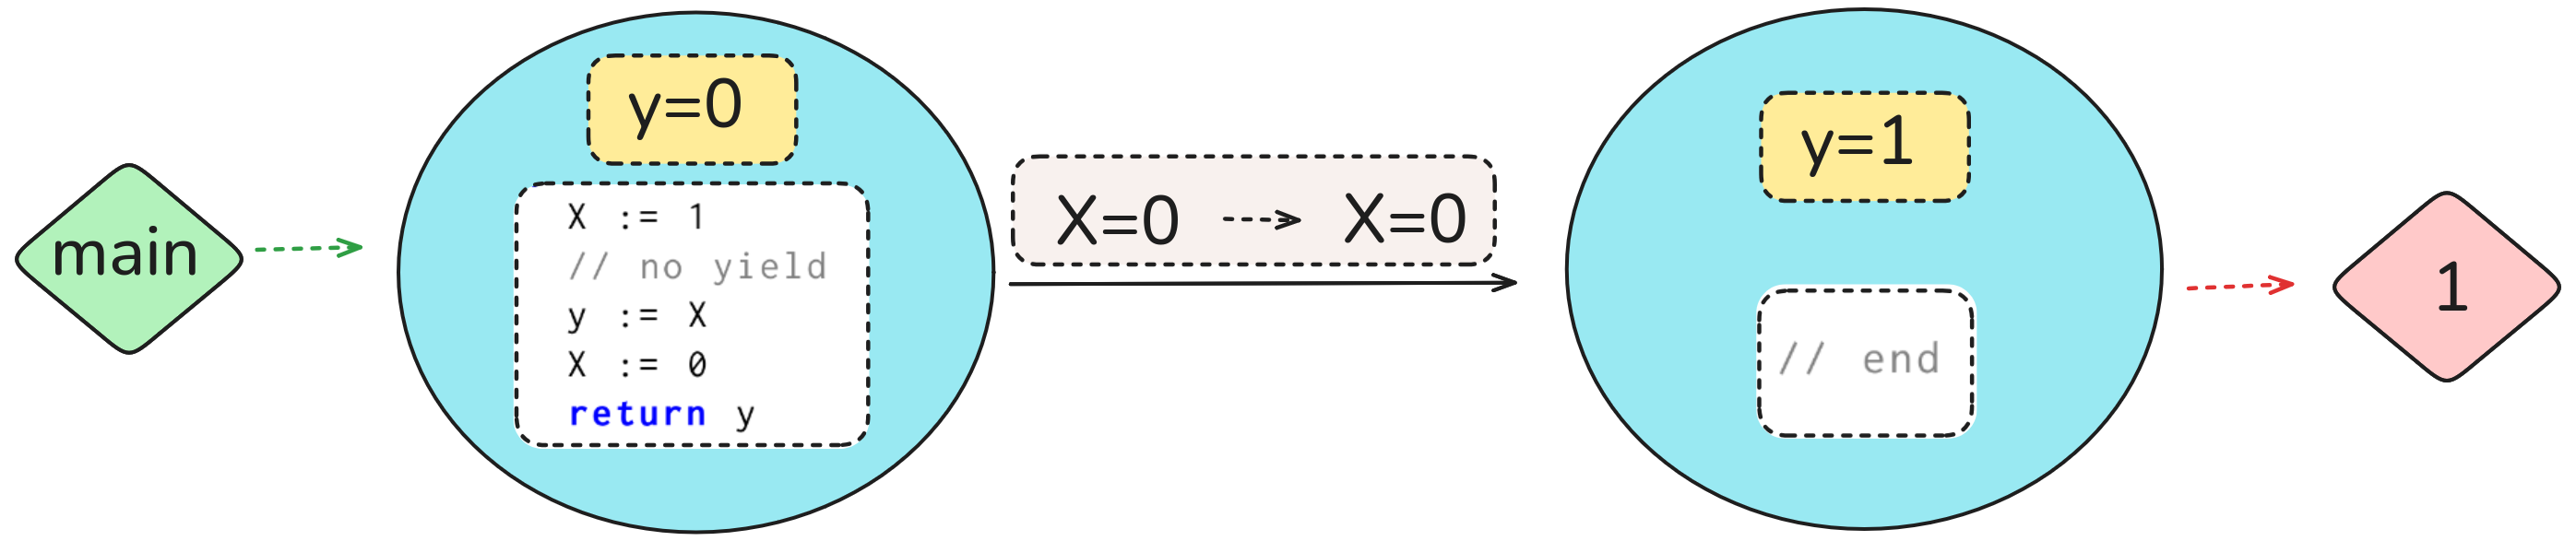
\includegraphics[width=0.9\textwidth]{plots/code_1_NS.png}
	\caption{Network System for interleaving executions of Listing~\ref{lst:MotivatingExample1Ser} program.}
	\label{fig:code1ExampleNS}
\end{figure}


\begin{figure}[htbp]
	\centering
	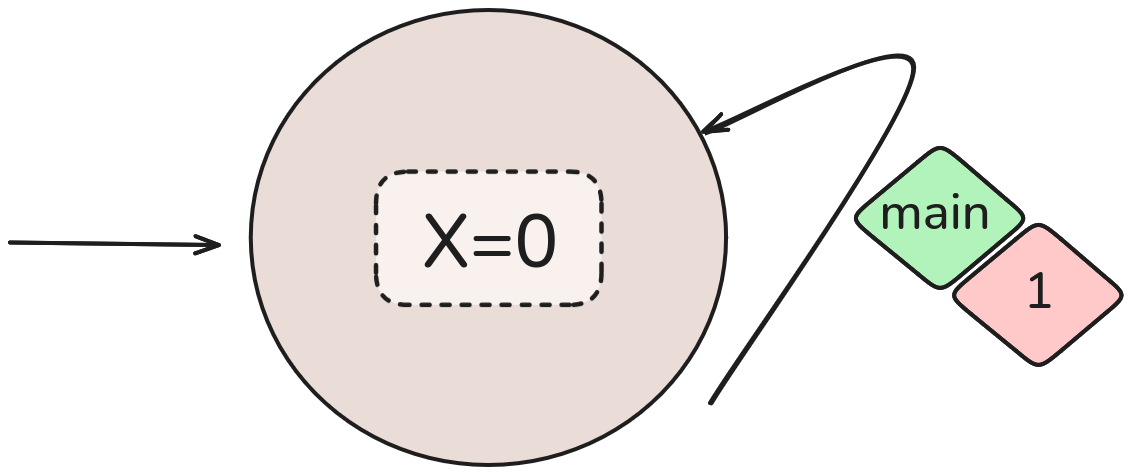
\includegraphics[width=0.35\textwidth]{plots/code_1_NFA.png}
	\caption{NFA for serialized executions of Listing~\ref{lst:MotivatingExample1Ser} program.}
	\label{fig:code1ExampleNFA}
\end{figure}



\begin{figure}[htbp]
	\centering
	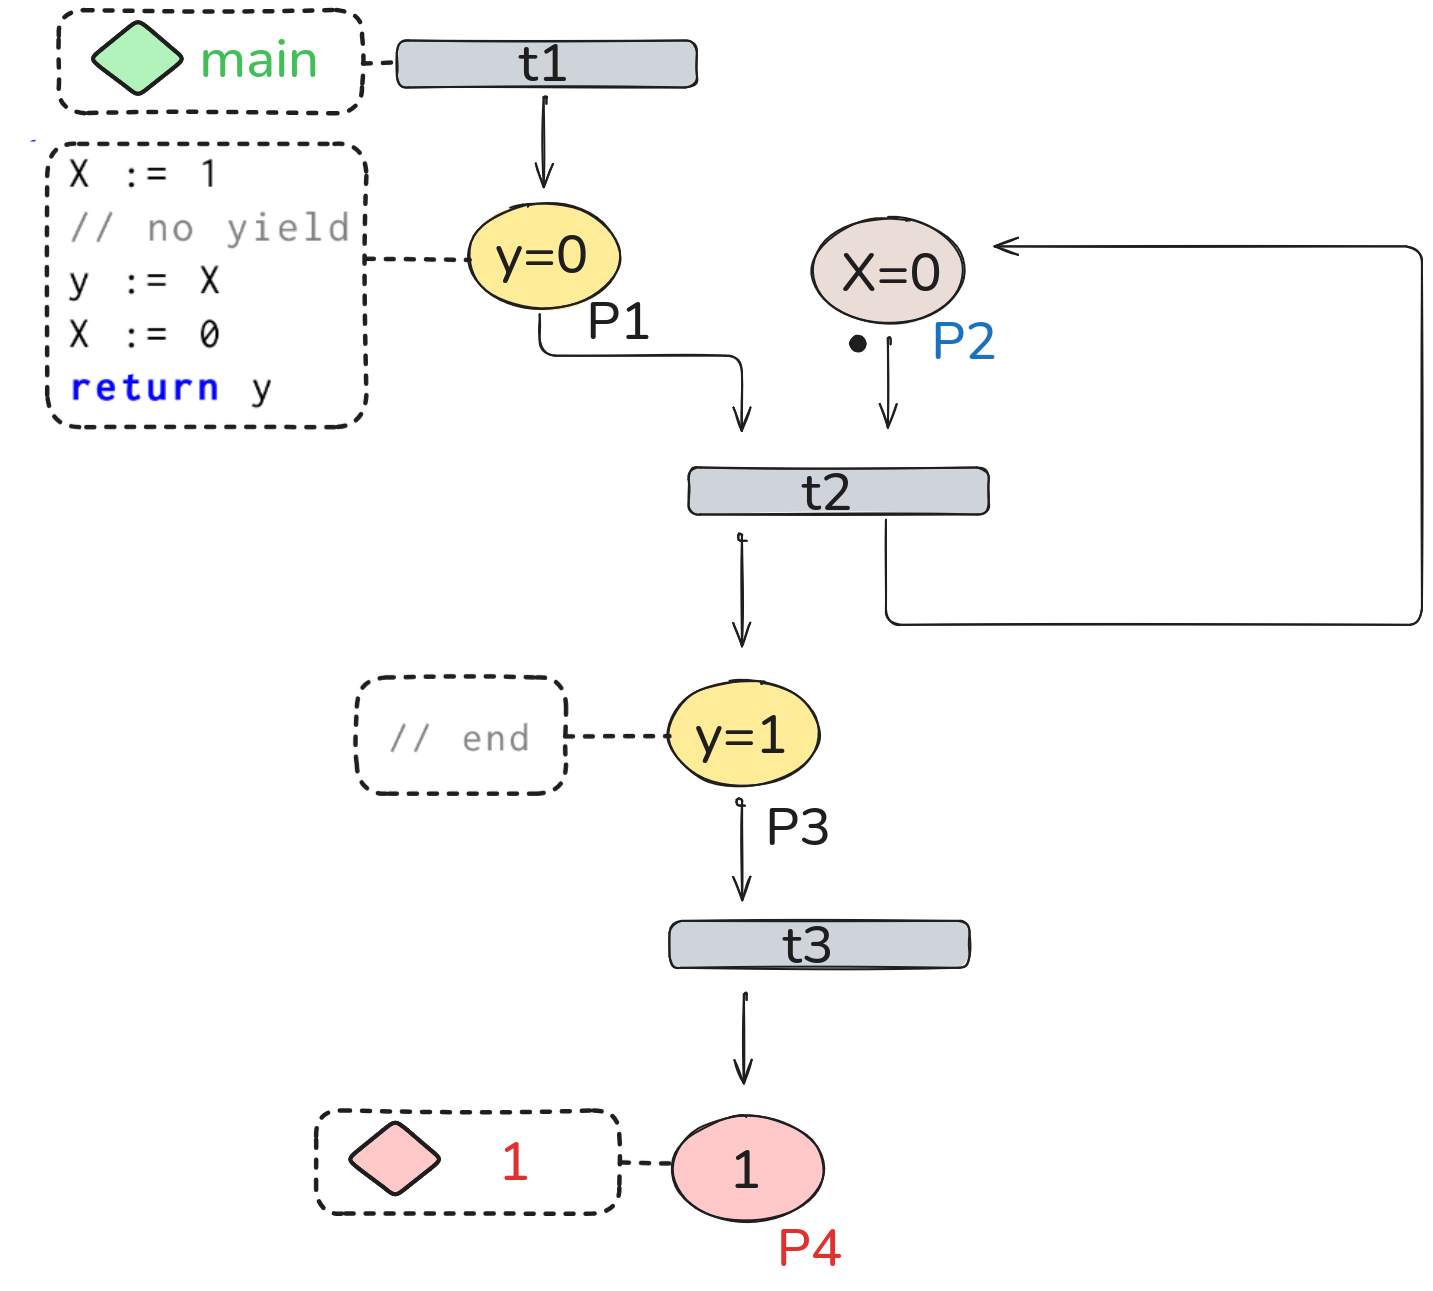
\includegraphics[width=0.5\textwidth]{plots/code_1_PN_with_annotation.png}
	\caption{Petri Net for interleaving executions of Listing~\ref{lst:MotivatingExample1Ser} program.}
	\label{fig:code1ExamplePN}
\end{figure}

%